\section{Plataforma Codeboard UERJ}

Este capítulo apresenta a plataforma Codeboard UERJ, que é uma ferramenta de apoio ao ensino de programação. Serão abordados os objetivos, funcionalidades e a arquitetura da plataforma.	


\subsection{Objetivos}

O objetivo principal da plataforma Codeboard UERJ é auxiliar no ensino de programação, permitindo que professores criem e gerenciem atividades práticas para seus alunos. A plataforma foi desenvolvida para ser utilizada em disciplinas de programação de computadores, como Algoritmos e Estruturas de Dados, Linguagens de Programação e Paradigmas de Programação.

A motivação para o desenvolvimento da plataforma surgiu durante a pandemia de COVID-19, quando as aulas presenciais foram suspensas e as atividades práticas de programação tiveram que ser adaptadas para o ensino remoto. Ela foi desenvolvida para atender a essa demanda, dando a capacidade aos professores de acompanharem o progresso dos alunos e avaliarem suas atividades práticas em tempo real.

\subsection{Funcionalidades}

Para atingir os objetivos propostos, o desenvolvimento da plataforma foi restrito a um conjunto de funcionalidades essenciais, que são:
Autenticação de usuários, gerenciamento de salas e seus participantes e o quadro de programação em tempo real.

\subsubsection{Autenticação de Usuários}

O sistema de autenticação de usuários é a primeira funcionalidade da plataforma. Ela permite que os usuários se cadastrem e façam login para acessar as funcionalidades da plataforma. O cadastro de usuários é feito através de um formulário que solicita nome, e-mail e senha. Após o cadastro, o usuário pode fazer login informando o e-mail e a senha cadastrados.

\begin{figure}[H]
    \centering
    \includegraphics[width=0.8\textwidth]{diagrams/user-auth-flow.png}
    \caption{Diagrama do fluxo de autenticação de usuários.}
    \label{fig:user-auth-flow}
\end{figure}

No processo de login, a plataforma verifica se o e-mail e a senha informados são válidos. Caso sejam, o usuário é autenticado e redirecionado para a tela inicial. Caso contrário, a plataforma exibe uma mensagem de erro informando que as credenciais são inválidas.

\begin{figure}[H]
    \centering
    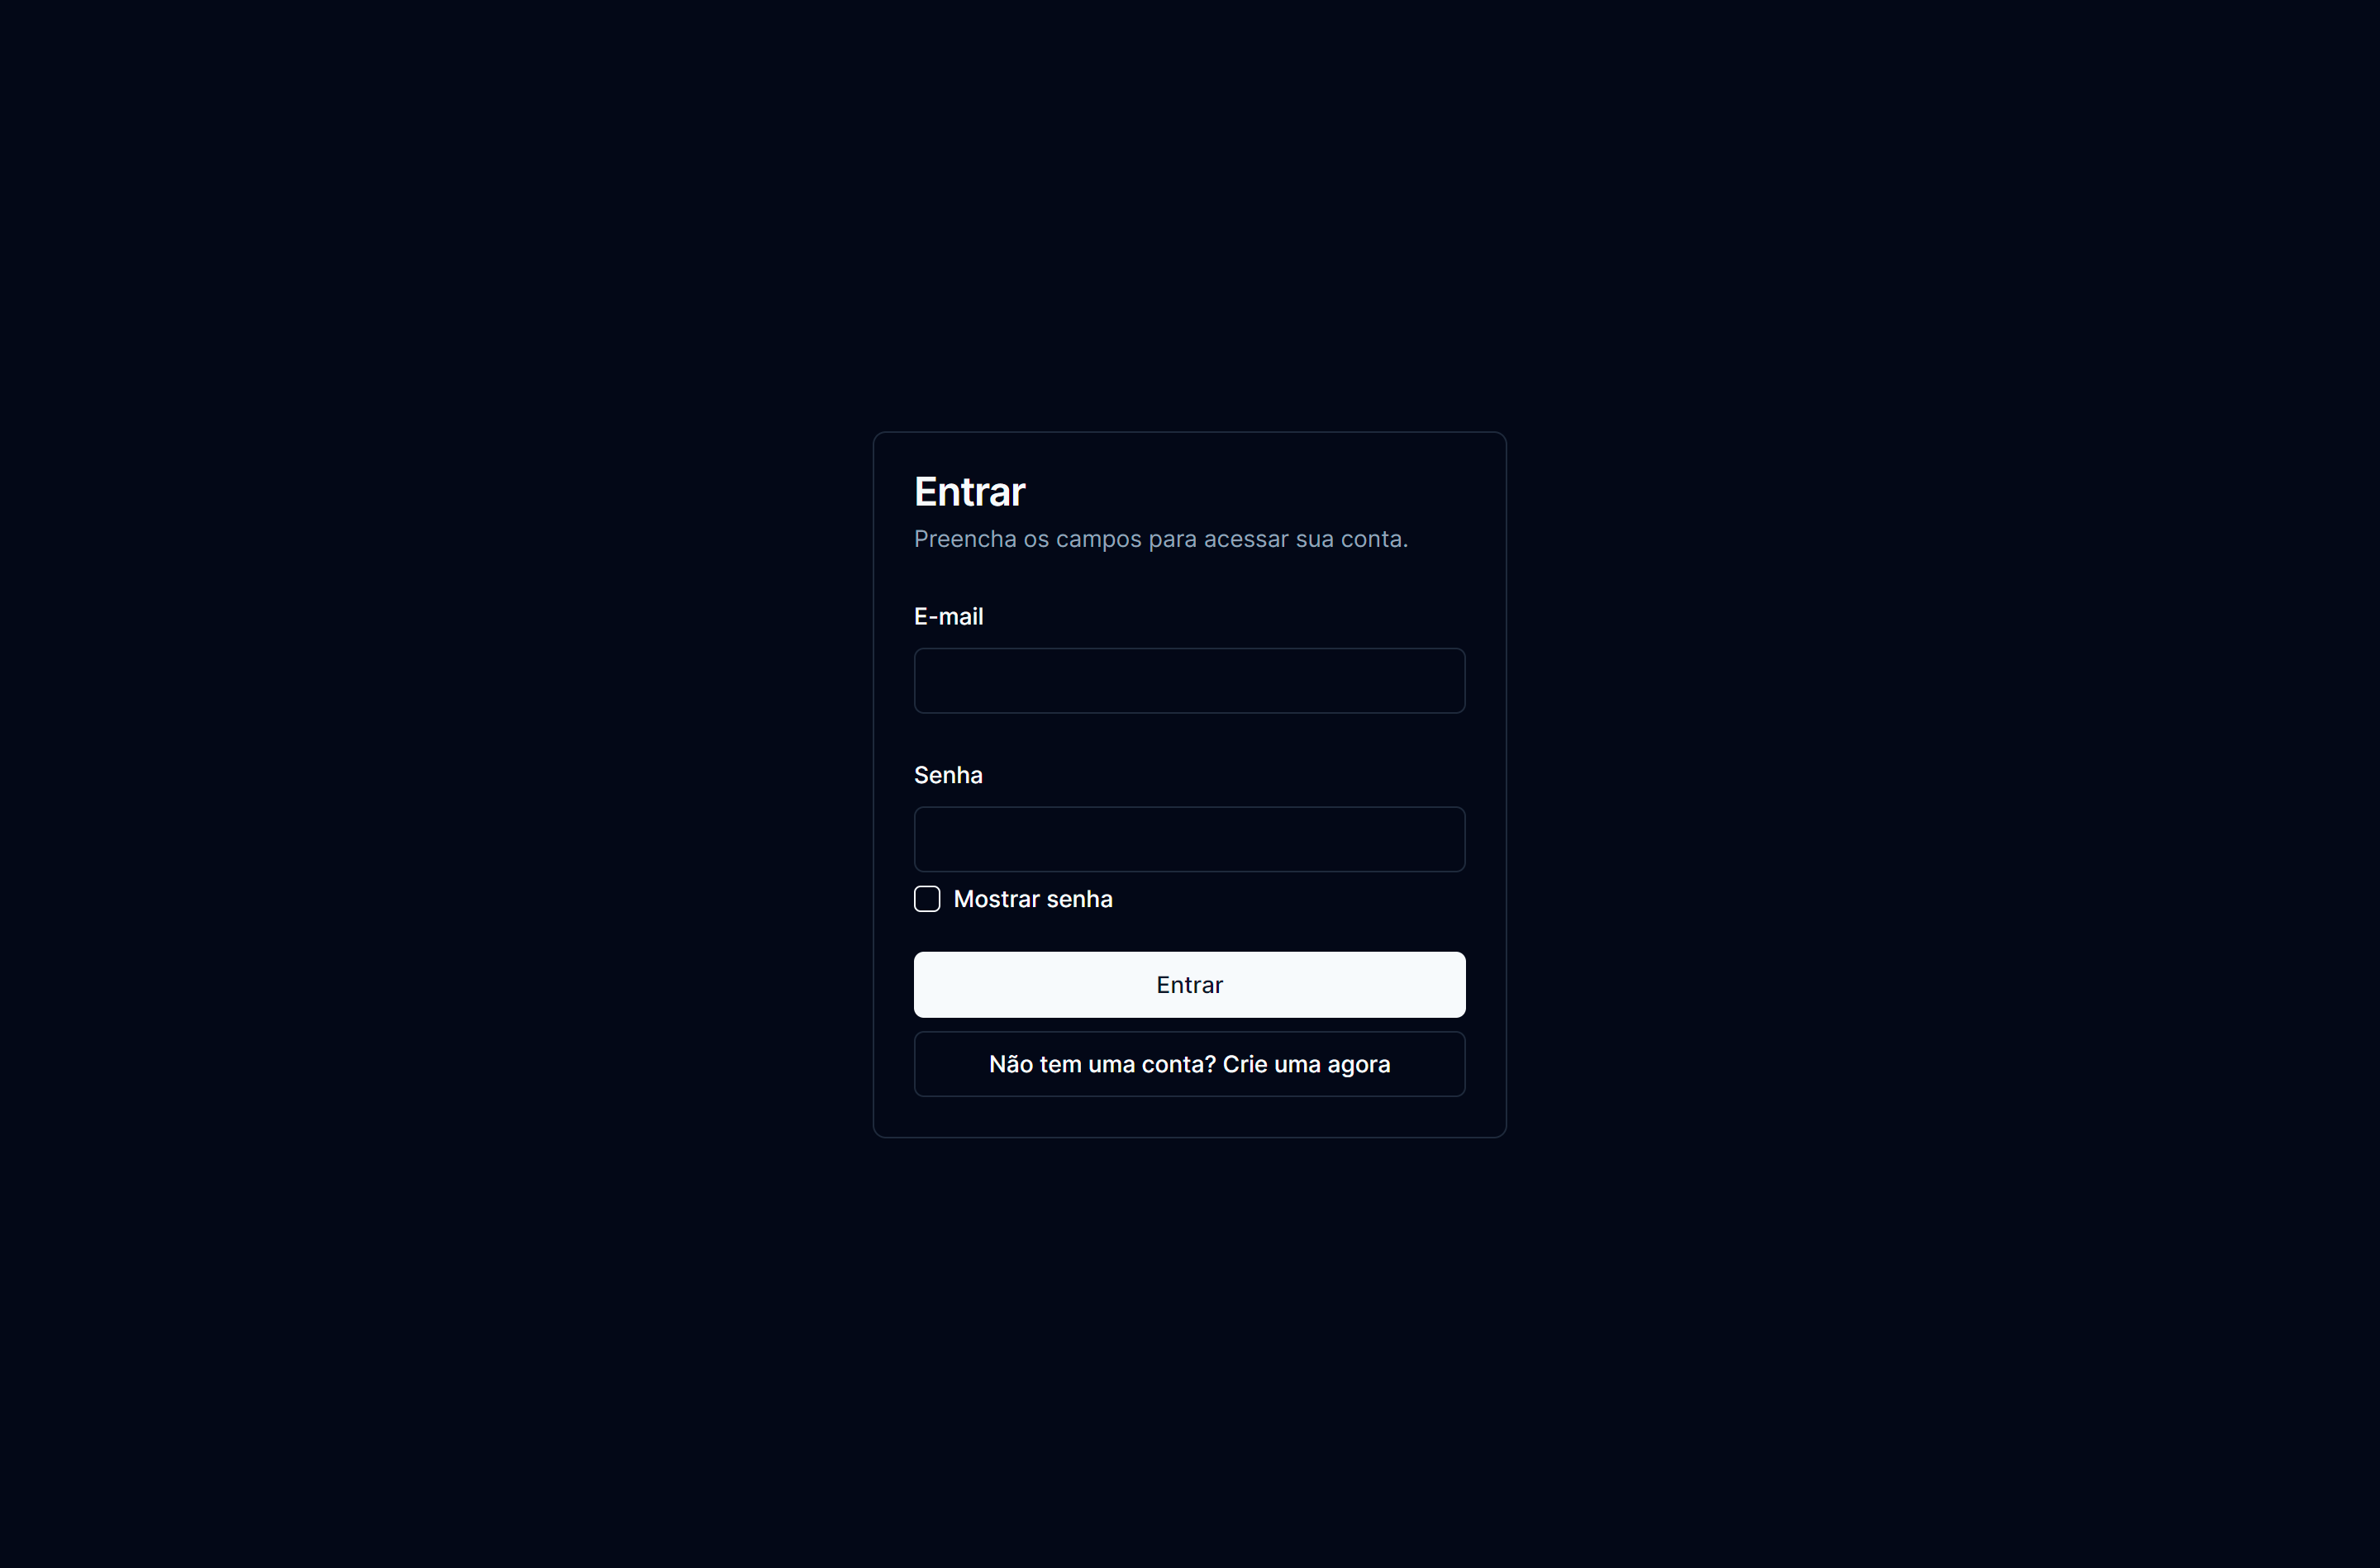
\includegraphics[width=0.8\textwidth]{assets/codeboard/login-page.png}
    \caption{Página de login da plataforma Codeboard UERJ.}
    \label{fig:login-page}
\end{figure}

No caso do usuário não possuir uma conta, ele pode clicar no link de cadastro e preencher o formulário de cadastro. Após o cadastro, o  usuário também é redirecionado para a tela inicial.

\begin{figure}[H]
    \centering
    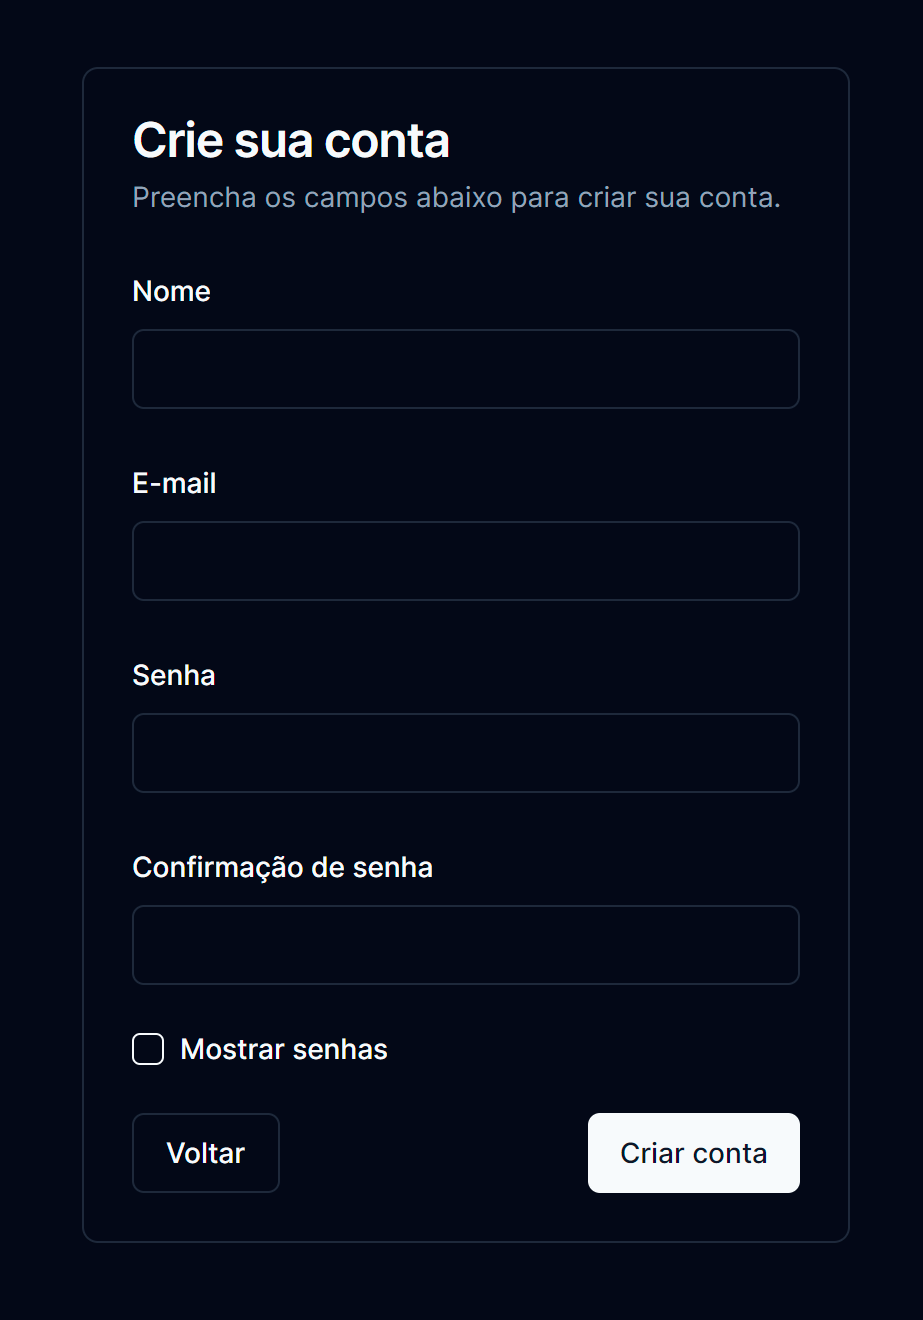
\includegraphics[width=0.8\textwidth]{assets/codeboard/signup-page.png}
    \caption{Página de cadastro da plataforma Codeboard UERJ.}
    \label{fig:signup-page}
\end{figure}

Durante o processo de autenticação, a plataforma utiliza tokens de autenticação para manter o usuário autenticado. O token é gerado no servidor e enviado para o cliente, onde é armazenado no navegador por meio de cookies. O token é utilizado para autenticar o usuário em todas as requisições feitas para o servidor, garantindo que o usuário esteja autenticado em todas as páginas da plataforma.

\subsubsection{Gerenciamento de Salas}

A funcionalidade de gerenciamento de salas permite que o professor crie, edite e acesse salas de aula. A criação de uma sala é feita através de um formulário que solicita o nome da sala e a descrição da atividade prática. Após a criação, o professor pode acessar a sala e adicionar alunos a ela.

\begin{figure}[H]
    \centering
    \includegraphics[width=0.8\textwidth]{diagrams/user-room-flow.png}
    \caption{Diagrama do fluxo de gerenciamento de salas.}
    \label{fig:user-room-flow}
\end{figure}

A tela de listagem de salas é a primeira tela exibida ao usuário após o login. Ela exibe todas as salas em que o usuário é dono ou membro. O usuário pode acessar uma sala clicando no botão de acesso, que o redireciona para a tela da sala.

\begin{figure}[H]
    \centering
    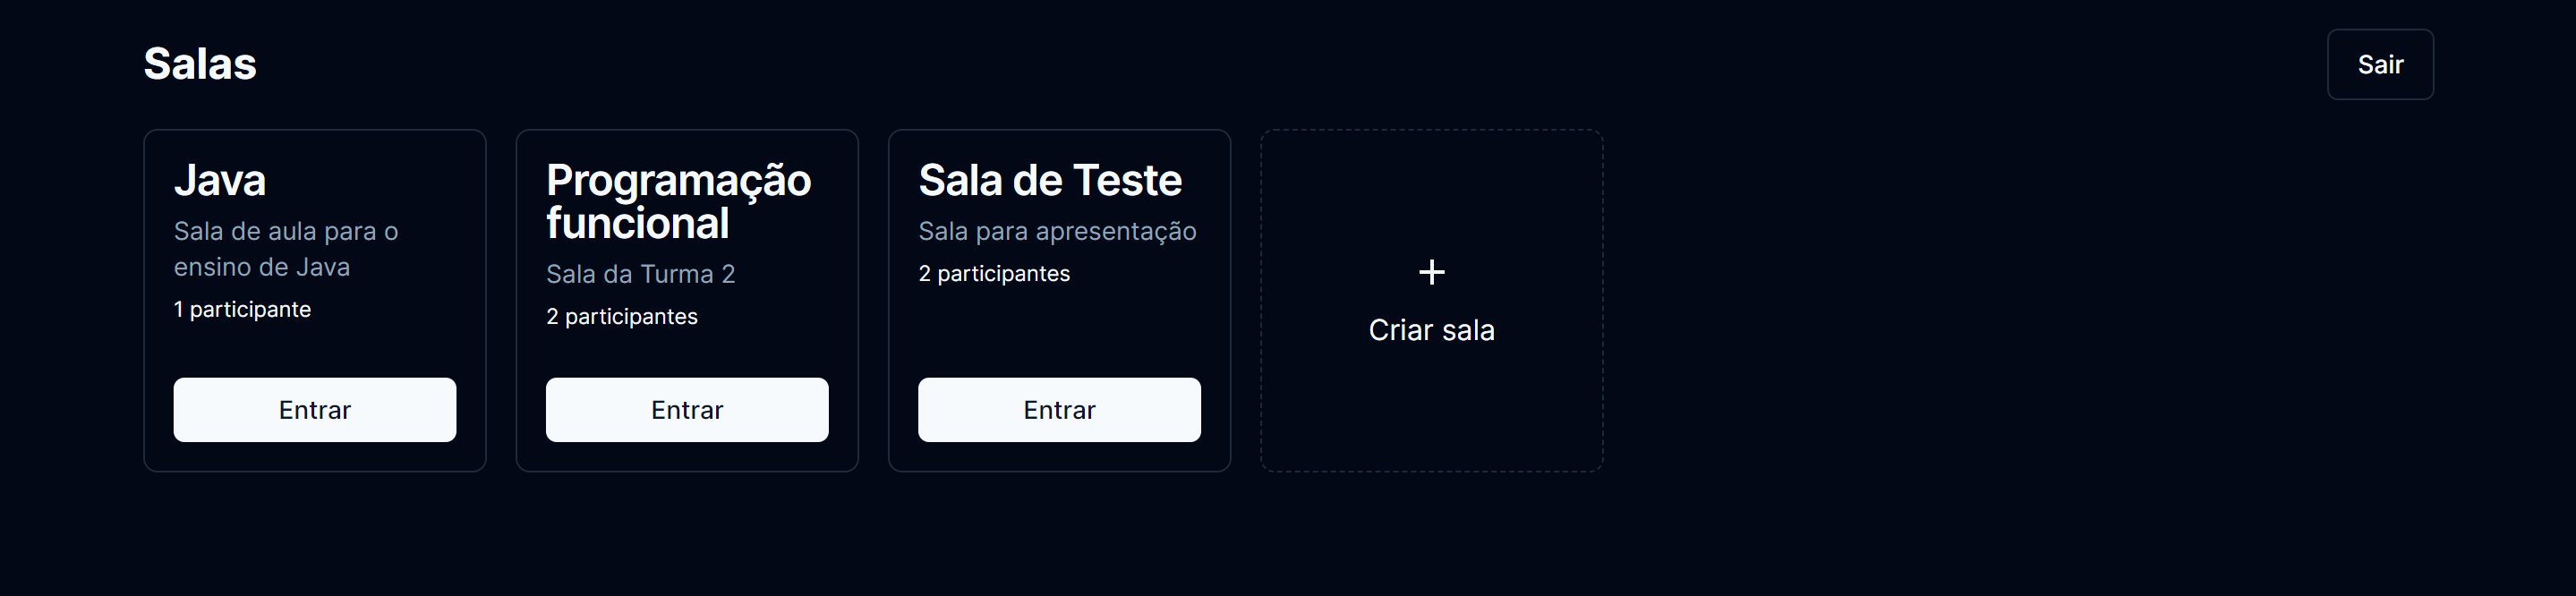
\includegraphics[width=0.8\textwidth]{assets/codeboard/rooms-page.png}
    \caption{Página de listagem de salas da plataforma Codeboard UERJ.}
    \label{fig:rooms-page}
\end{figure}

Nesta mesma tela da figura \ref{fig:rooms-page}, o usuário pode criar uma nova sala clicando no botão de criação de sala. O usuário é redirecionado para uma tela de criação de sala, onde ele pode preencher o nome e a descrição da sala. Após a criação, o usuário é redirecionado para a tela da sala.

\begin{figure}[H]
    \centering
    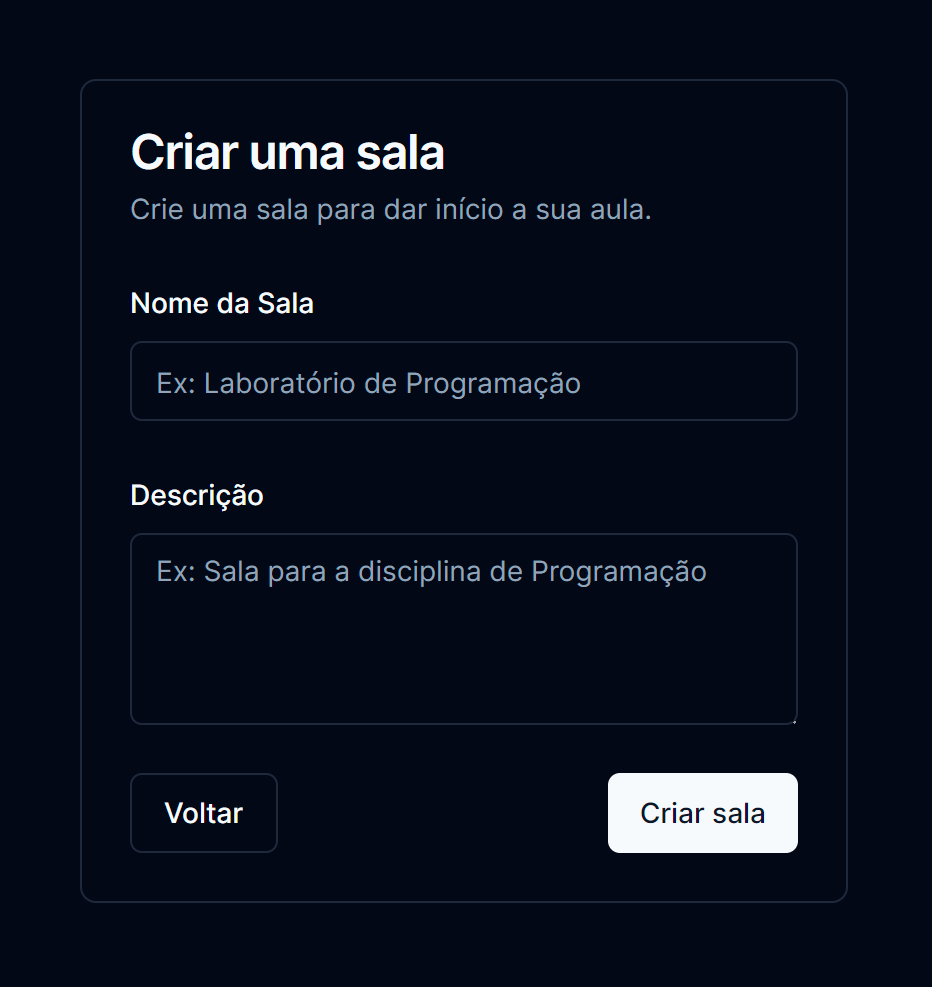
\includegraphics[width=0.8\textwidth]{assets/codeboard/create-room-page.png}
    \caption{Página de criação de sala da plataforma Codeboard UERJ.}
    \label{fig:create-room-page}
\end{figure}

Para adicionar alunos à sala, o usuário pode clicar num botão de adição de membros representado por um ícone de usuário. A plataforma exibe um modal com um campo de e-mail, onde o usuário pode informar o e-mail do aluno que deseja adicionar à sala. Após a adição, o aluno se torna membro da sala e pode acessá-la.

\begin{figure}[H]
    \centering
    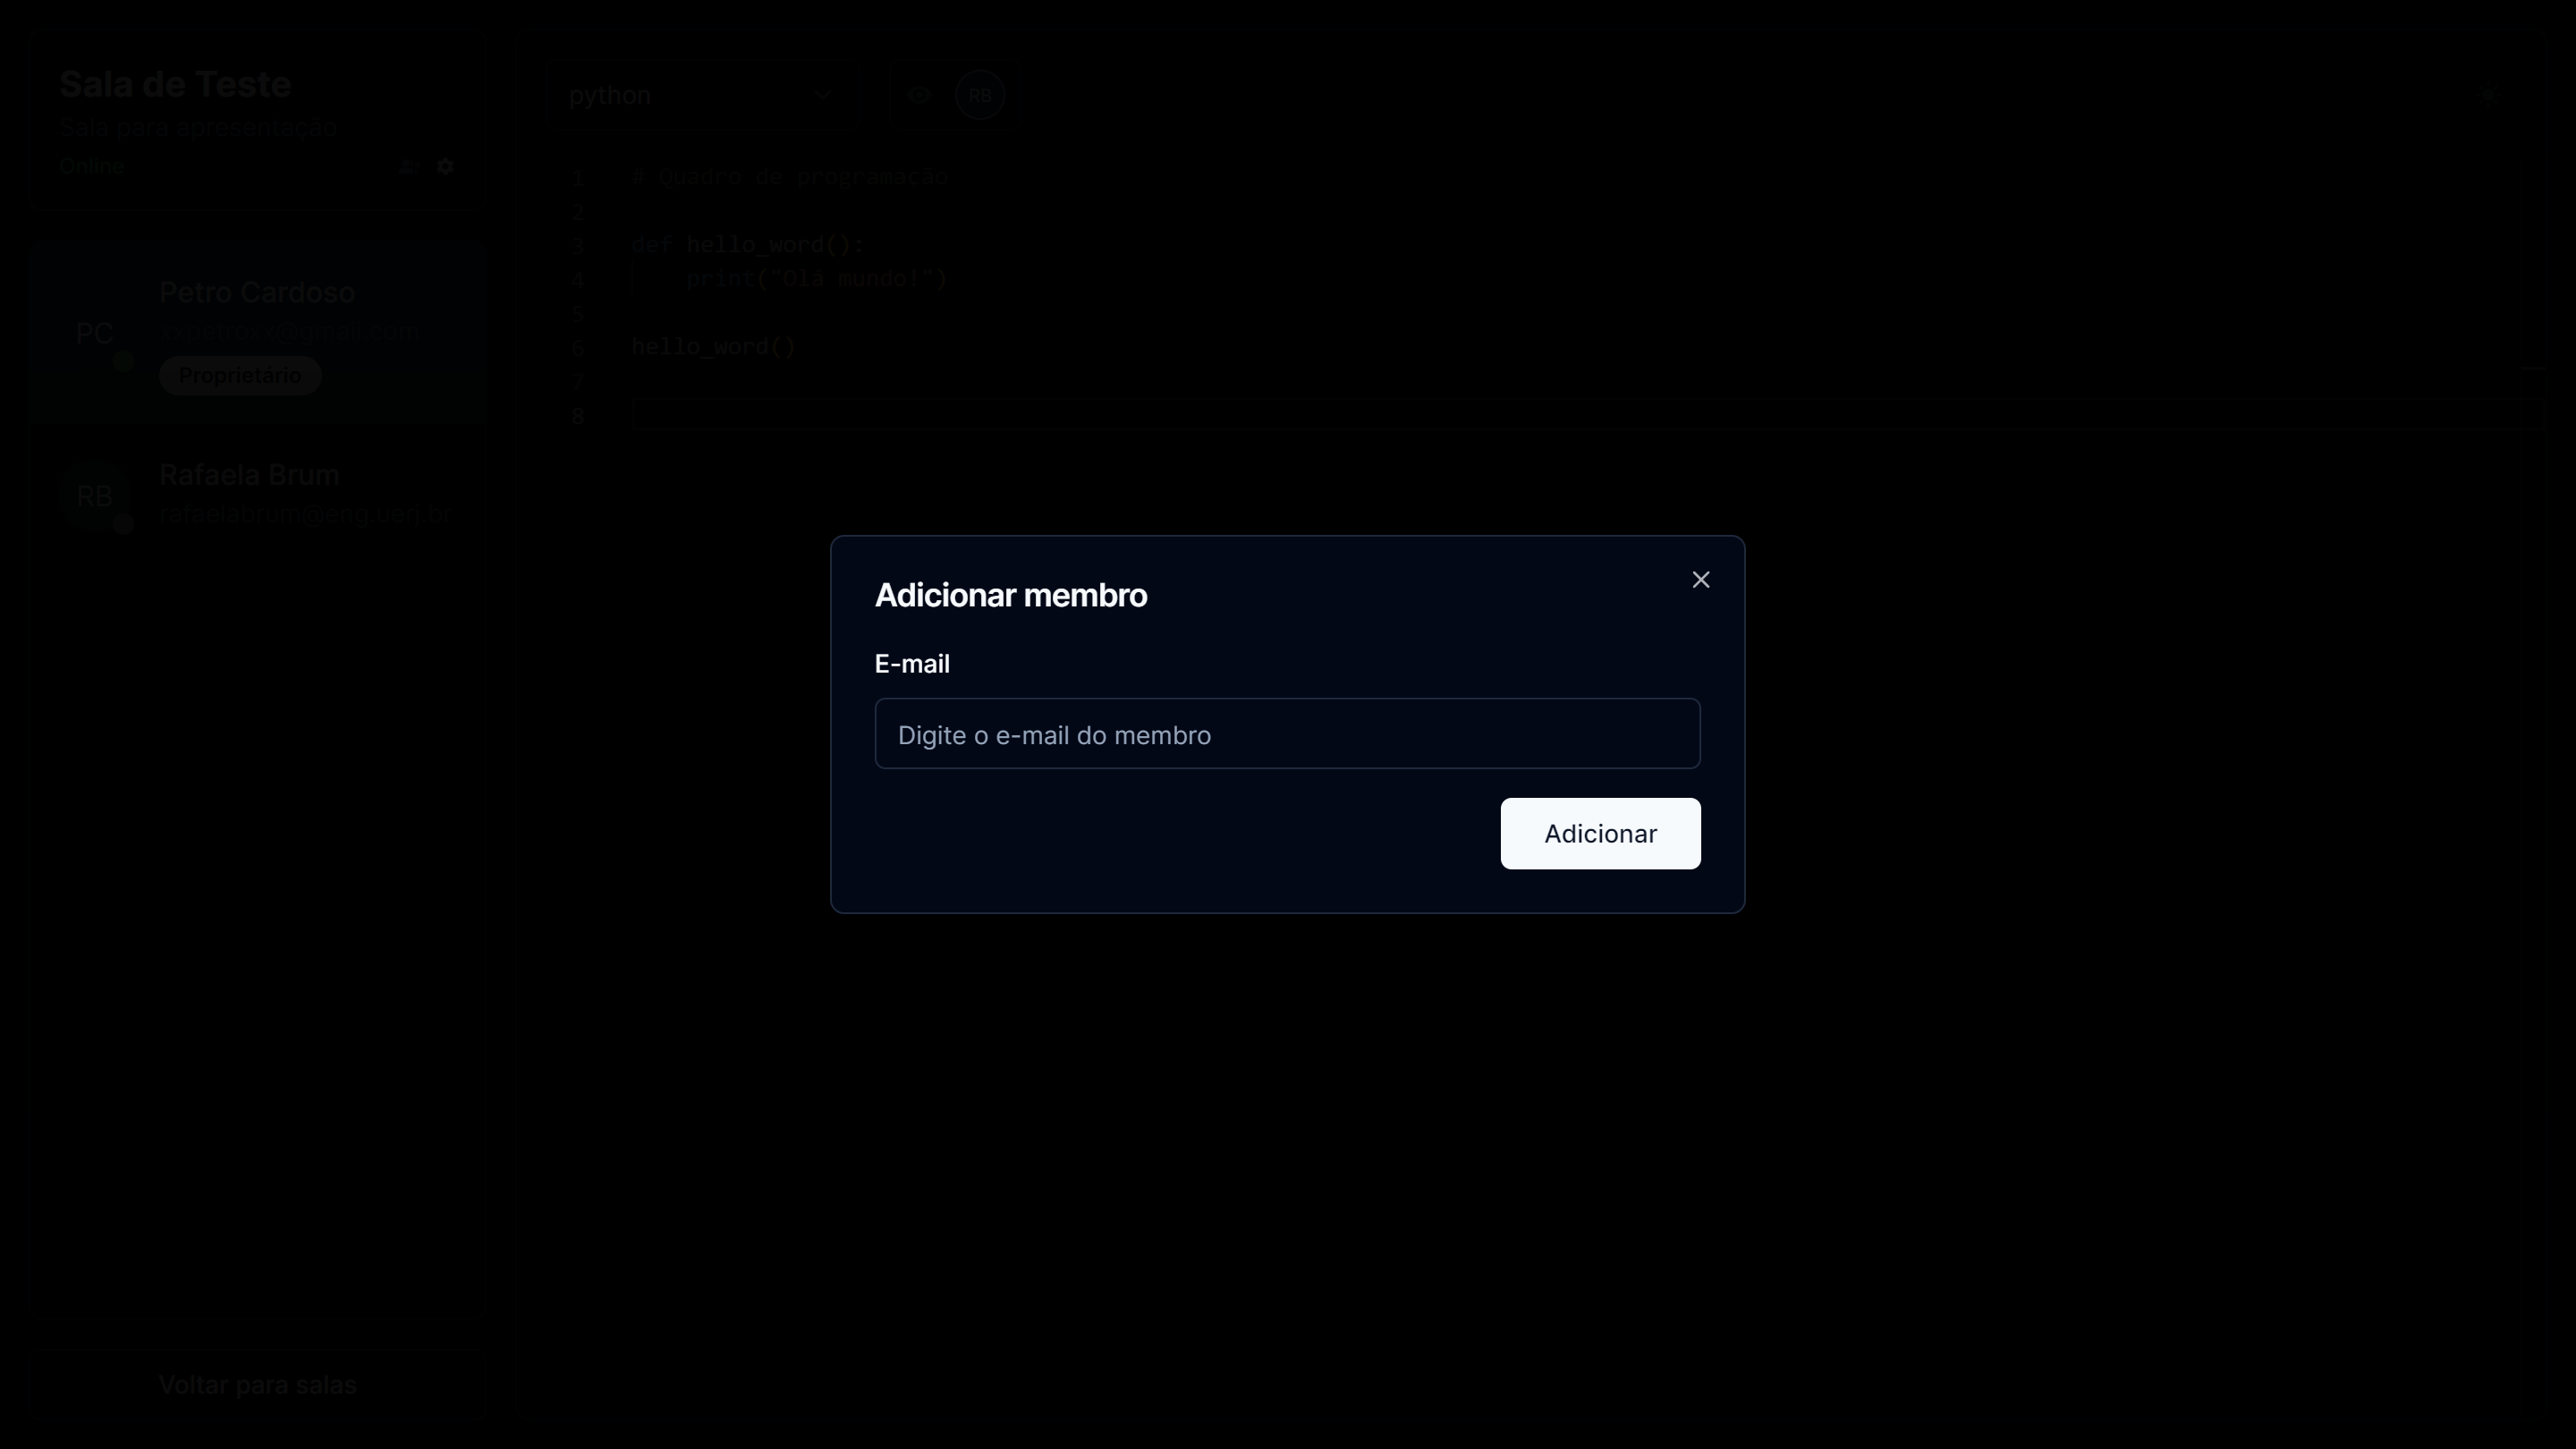
\includegraphics[width=0.8\textwidth]{assets/codeboard/add-member-modal.png}
    \caption{Página de adição de alunos à sala da plataforma Codeboard UERJ.}
    \label{fig:add-member-modal}
\end{figure}

\subsubsection{Quadro de Programação em Tempo Real}

A funcionalidade de quadro de programação em tempo real é a principal funcionalidade da plataforma. Ela permite que os alunos escrevam códigos de programação diretamente no navegador, sem a necessidade de instalar um ambiente de desenvolvimento integrado (IDE).

Para acessar o quadro de programação, o usuário deve acessar a sala desejada. A plataforma exibe uma tela dividida em dois módulos, o módulo lateral de seleção de usuário e o módulo central de edição de código.

\begin{figure}[H]
    \centering
    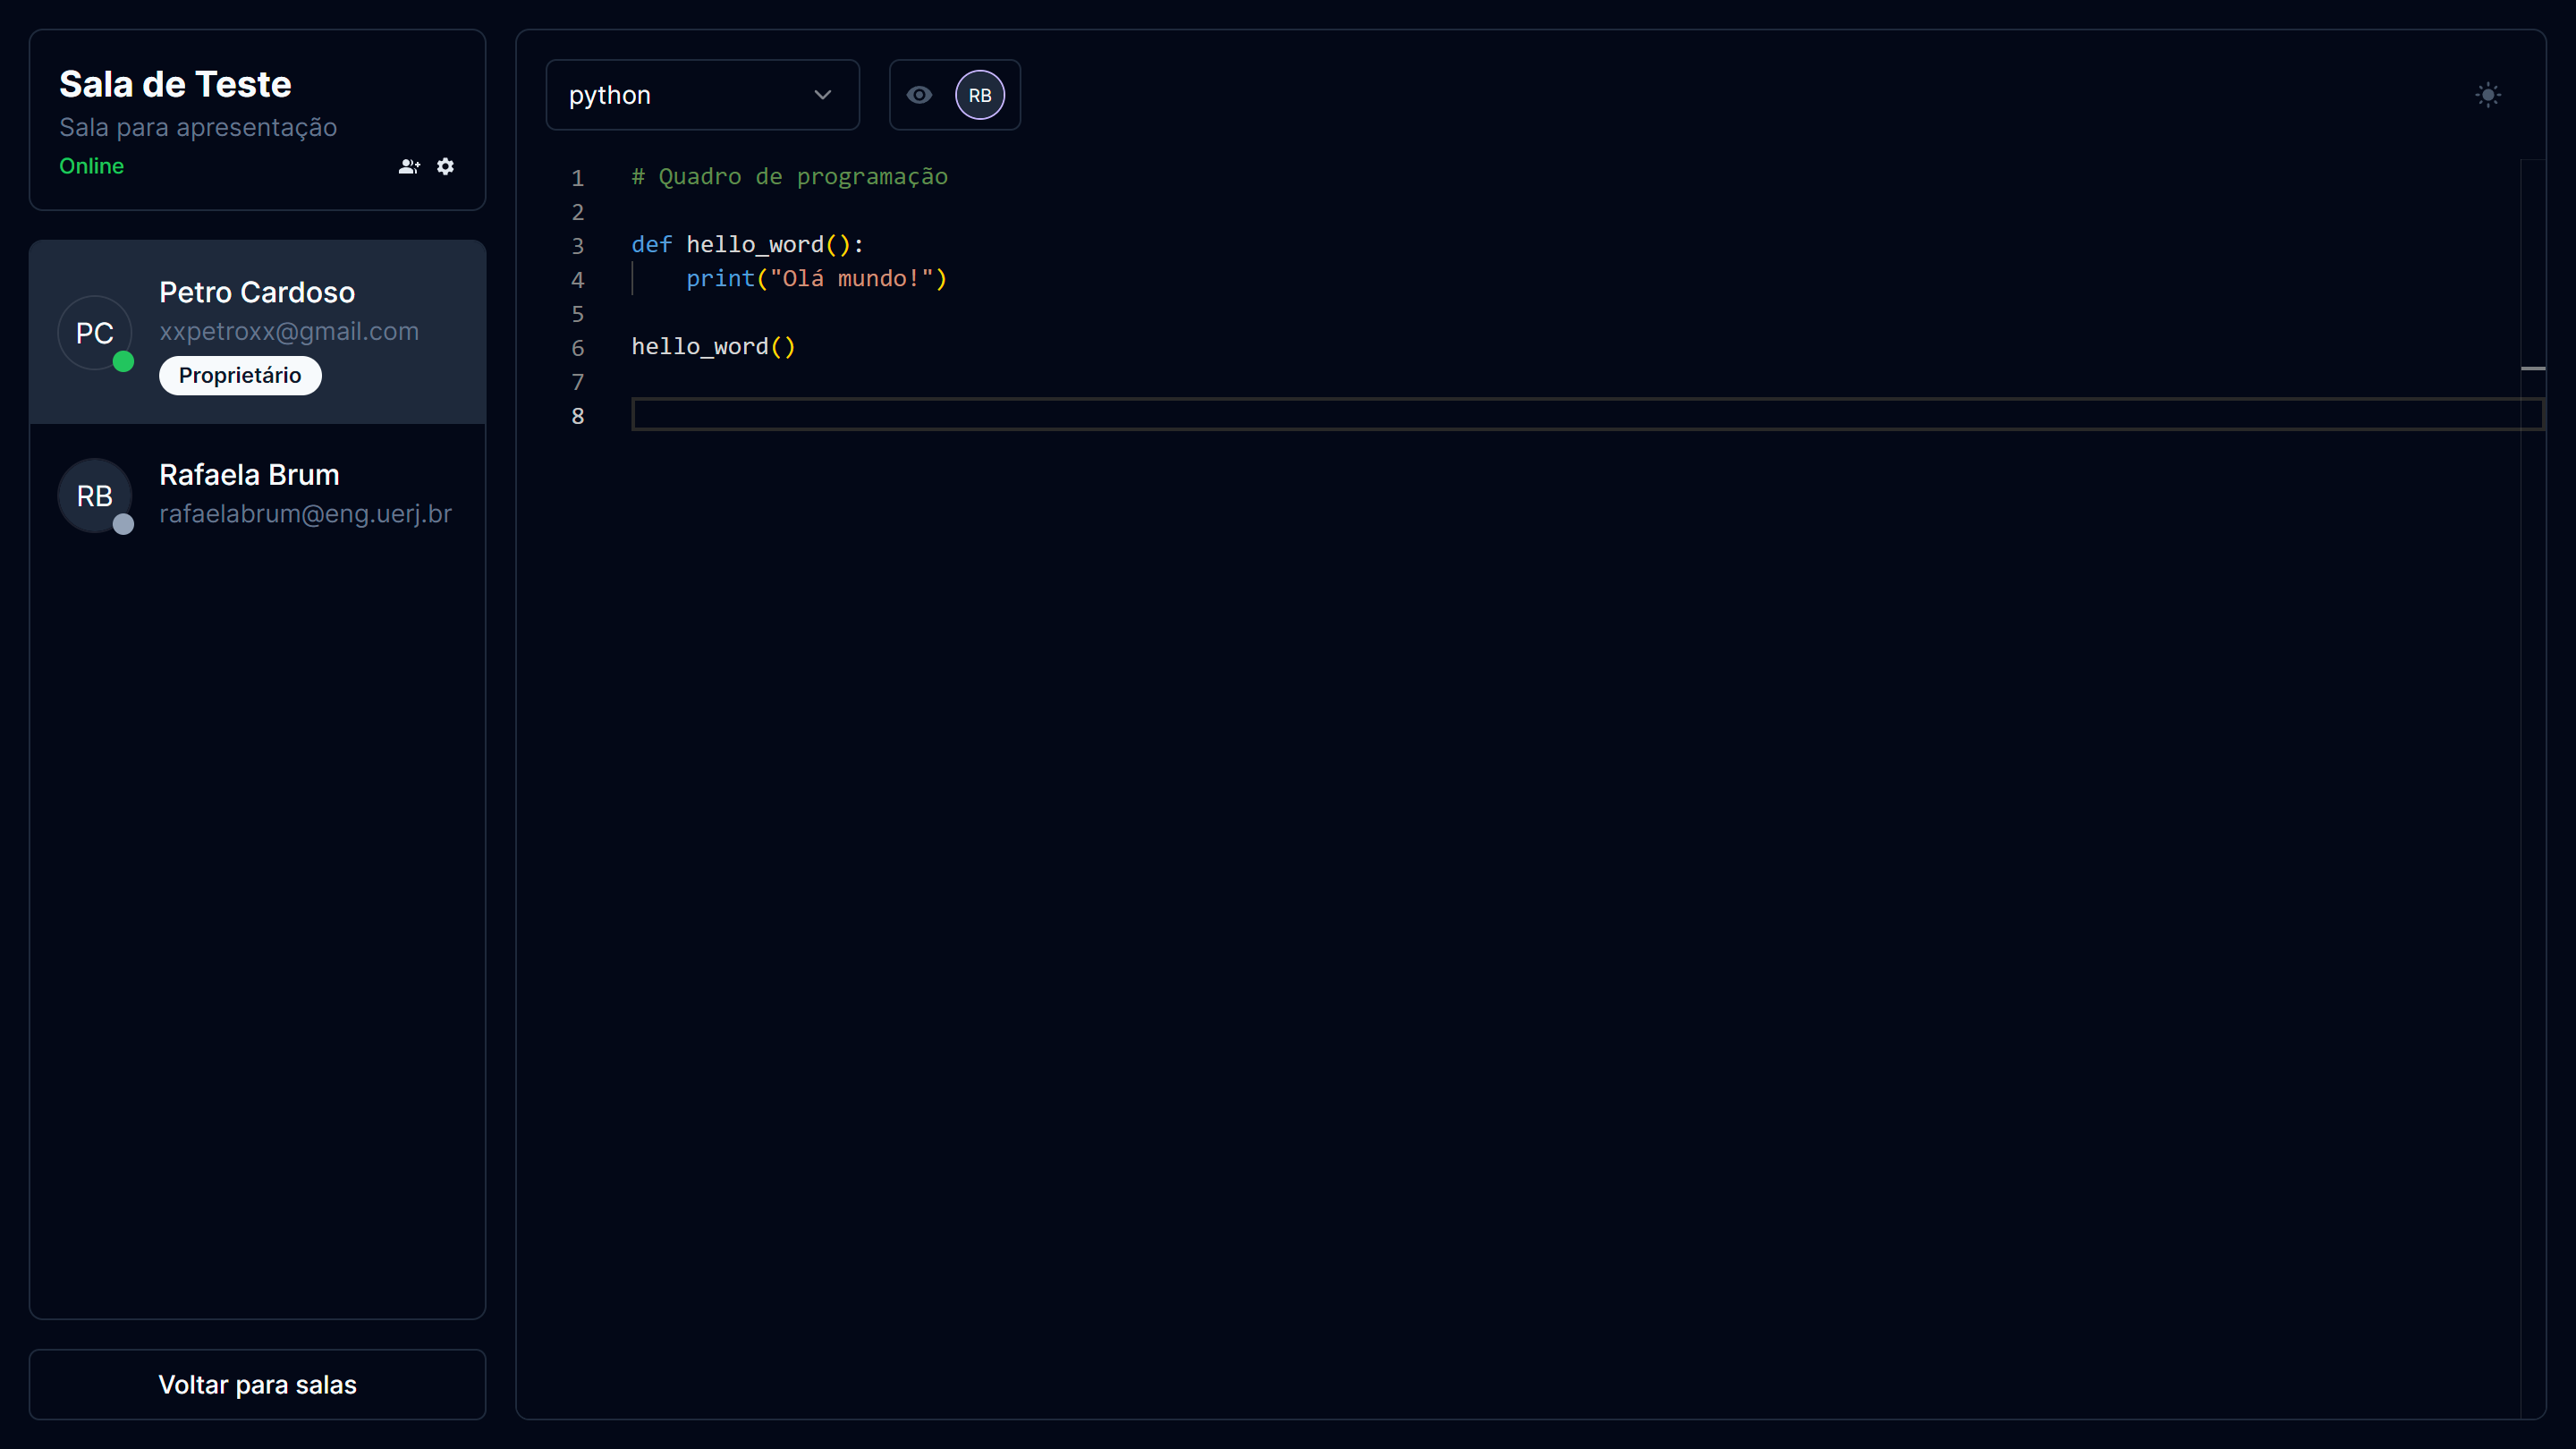
\includegraphics[width=0.8\textwidth]{assets/codeboard/room-details-page.png}
    \caption{Página da sala de programação da plataforma Codeboard UERJ.}
    \label{fig:room-details-page}
\end{figure}


Como mostra a figura \ref{fig:room-details-page}, o módulo lateral exibe a lista de membros da sala. Para cada membro listado, é exibido o nome, a foto de perfil e indicadores para caso ele esteja online ou esteja editando o seu próprio código. O usuário pode selecionar outro membro da sala na lista lateral para visualizar e interagir com o código dele.

Caso o usuário já esteja com si mesmo selecionado, ele poderá editar o próprio código, trocar de linguagem de programação e visualizar quem está visualizando seu código. O código é salvo automaticamente a cada edição realizada pelo usuário.

Acima do módulo lateral, a plataforma exibe o nome da sala e sua descrição. Caso o usuário seja o dono da sala, também serão exibidos os botões de adição de membros e de configuração da sala. O botão de adição de membros permite que o usuário adicione novos membros à sala, enquanto o botão de configuração permite que o usuário edite o nome e a descrição da sala.

\begin{figure}[H]
    \centering
    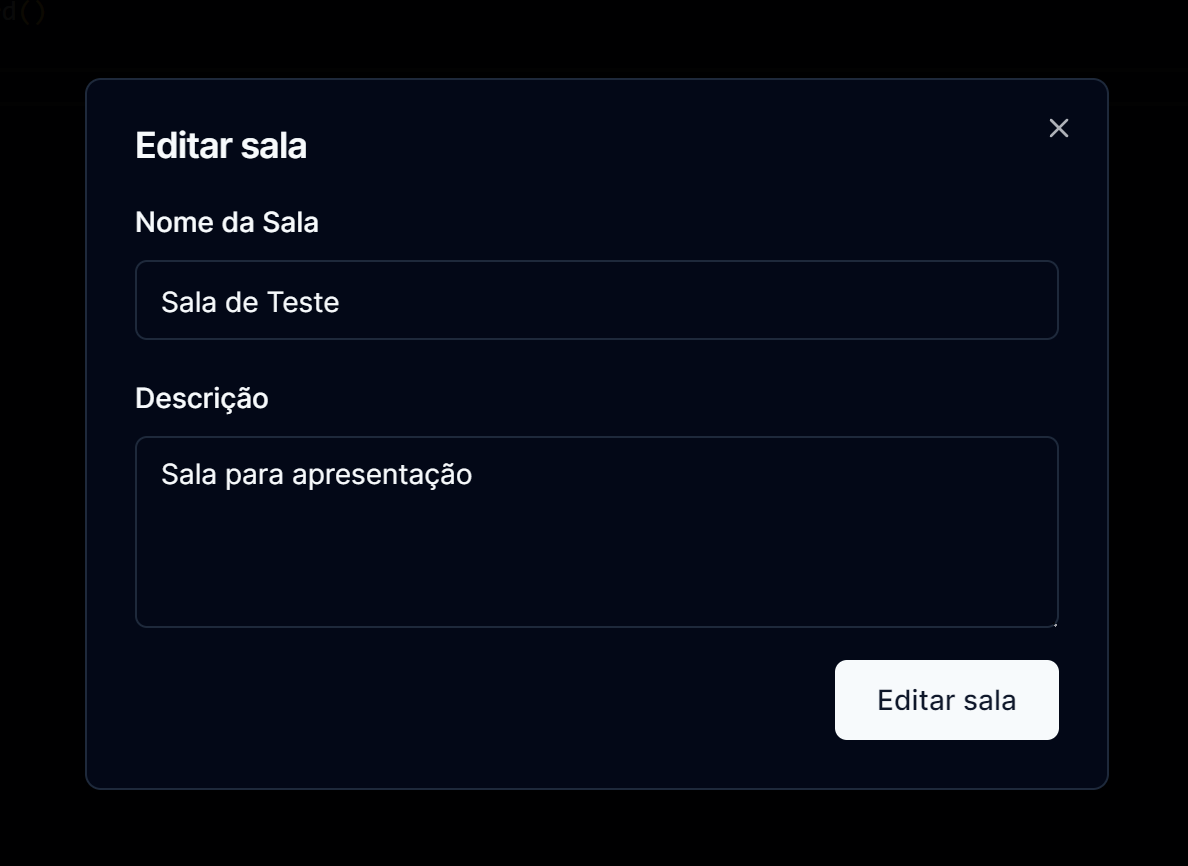
\includegraphics[width=0.8\textwidth]{assets/codeboard/edit-room-modal.png}
    \caption{Modal de configuração de sala da plataforma Codeboard UERJ.}
    \label{fig:edit-room-modal}
\end{figure}


Abaixo do módulo lateral, a plataforma exibe um botão de saída da sala. Ao clicar neste botão, o usuário é redirecionado para a tela de listagem de salas, onde ele pode acessar outras salas ou criar uma nova sala.

O módulo central exibe o editor de código. Este editor suporta as funcionalidades básicas de um IDE, como coloração de sintaxe, auto-completar e formatação de código. Durante a visualização do código de outro usuário, o usuário pode somente fazer marcações que são exibidas em tempo real para o outros usuários presentes no quadro.

% Foto da marcação de código

Na parte superior do editor, o usuário pode selecionar a linguagem de programação desejada. A plataforma suporta as linguagens de programação mais utilizadas, como C, C++, Java, Python, JavaScript, entre outras. A seleção da linguagem de programação altera a coloração de sintaxe do editor, facilitando a escrita e a leitura do código.

% Foto da parte superior do editor

Ao lado da seleção de linguagem, o usuário pode visualizar quem está visualizando o seu código no momento. A plataforma exibe uma lista horizontal com estes visualizadores, permitindo que ele saiba quem está acompanhando o seu progresso.


\subsection{Arquitetura}

To do

\subsubsection{Backend}

To do

\subsubsection{Banco de Dados}

To do 


\subsubsection{Frontend}

To do

\subsubsection{Comunicação via REST API}

To do

\subsubsection{Comunicação em Tempo Real}

To do
